\documentclass[aspectratio=169]{beamer}

\usetheme{Madrid}
\usecolortheme{default}

\usepackage[utf8]{inputenc}
\usepackage[T1]{fontenc}
\usepackage{array}
\usepackage{booktabs}
\usepackage{graphicx}
\usepackage{tikz}
\usepackage{xcolor}

\usetikzlibrary{arrows.meta,positioning}

\definecolor{projectblue}{RGB}{24, 48, 82}
\definecolor{projectgold}{RGB}{191, 132, 48}
\definecolor{projectgreen}{RGB}{42, 117, 93}
\definecolor{projectred}{RGB}{166, 61, 64}
\definecolor{softgray}{RGB}{245, 247, 250}
\definecolor{inkgray}{RGB}{42, 48, 56}

\setbeamercolor{structure}{fg=projectblue}
\setbeamercolor{frametitle}{fg=projectblue}
\setbeamercolor{title}{fg=projectblue}
\setbeamercolor{subtitle}{fg=inkgray}
\setbeamercolor{block title}{bg=projectblue, fg=white}
\setbeamercolor{block body}{bg=softgray, fg=black}
\setbeamercolor{alerted text}{fg=projectred}
\setbeamertemplate{navigation symbols}{}

\setbeamertemplate{footline}{%
  \leavevmode%
  \hbox{%
    \begin{beamercolorbox}[wd=.76\paperwidth,ht=2.3ex,dp=1ex,leftskip=1em]{author in head/foot}%
      \small Towards Accessible OMR
    \end{beamercolorbox}%
    \begin{beamercolorbox}[wd=.24\paperwidth,ht=2.3ex,dp=1ex,rightskip=1em plus1fil]{date in head/foot}%
      \hfill\small \insertframenumber/\inserttotalframenumber
    \end{beamercolorbox}%
  }%
}

\graphicspath{{samples/}{samples/stage_outputs/}}

\newcommand{\maybeimage}[2][]{%
  \IfFileExists{#2}{%
    \includegraphics[#1]{#2}%
  }{%
    \fbox{\parbox[c][0.28\textheight][c]{0.72\linewidth}{\centering Missing image: \texttt{#2}}}%
  }%
}

\newcommand{\metric}[2]{%
  \begin{block}{#1}
    \centering\Large #2
  \end{block}
}

\title[Accessible OMR]{Towards Accessible Optical Mark Recognition}
\subtitle{A Classical Computer Vision Baseline for Answer-Sheet Grading}
\author{Oween}
\institute{%
  Technische Hochschule Deggendorf\\
  Artificial Intelligence B. Sc.\\
  Computer Vision Final Project
}
\date{\today}

\begin{document}

\begin{frame}
  \titlepage
\end{frame}

\begin{frame}{Why This Problem Matters}
  \begin{block}{Motivation}
    In many low-resource schools, teachers still grade multiple-choice exams by hand. The work is repetitive, slow, and takes time away from feedback, preparation, and student support.
  \end{block}

  \vspace{0.25cm}

  \begin{columns}[T]
    \begin{column}{0.52\textwidth}
      \textbf{Project idea}
      \begin{itemize}
        \item Use ordinary scanned answer sheets.
        \item Avoid expensive dedicated OMR hardware.
        \item Build an explainable grading assistant.
        \item Keep uncertain cases visible for human review.
      \end{itemize}
    \end{column}
    \begin{column}{0.42\textwidth}
      \centering
      \maybeimage[height=0.58\textheight]{samples/File0005.jpg}
    \end{column}
  \end{columns}
\end{frame}

\begin{frame}{Research Question}
  \begin{block}{Main question}
    Can we build a low-cost and explainable OMR pipeline that detects answer-sheet regions, extracts marked bubbles, and prepares reliable grading outputs from scanned exam images?
  \end{block}

  \vspace{0.2cm}

  \textbf{Current scope}
  \begin{itemize}
    \item Classical image-processing pipeline up to bubble detection.
    \item Method 1: rule-based interpretation and grading.
    \item Human-review labels for unclear or multiple-mark answers.
  \end{itemize}

  \vspace{0.15cm}

  \textbf{Later scope}
  \begin{itemize}
    \item Compare the classical baseline with AI-based mark detection.
    \item Test robustness across templates, mark styles, and scan quality.
  \end{itemize}
\end{frame}

\begin{frame}{Why This Fits an AI Project}
  \begin{columns}[T]
    \begin{column}{0.48\textwidth}
      \textbf{Classical vision first}
      \begin{itemize}
        \item transparent thresholds,
        \item visible intermediate outputs,
        \item explainable failure cases,
        \item strong baseline before ML.
      \end{itemize}
    \end{column}
    \begin{column}{0.48\textwidth}
      \textbf{AI comparison later}
      \begin{itemize}
        \item learned mark detector,
        \item possible CNN or object detector,
        \item comparison against Method 1,
        \item accuracy, review rate, and runtime.
      \end{itemize}
    \end{column}
  \end{columns}

  \vspace{0.35cm}

  \begin{block}{Design principle}
    The AI part becomes stronger when the classical baseline is measurable, reproducible, and honestly evaluated.
  \end{block}
\end{frame}

\begin{frame}{Reference Method}
  \begin{block}{Paper inspiration}
    The reference paper proposes an unsupervised OMR pipeline for scanned multiple-choice answer sheets. Its practical core is a staged process: locate reference rectangles, normalize the sheet, identify option circles, and assign answer values.
  \end{block}

  \begin{itemize}
    \item detect ID and answer-section rectangles,
    \item apply perspective correction,
    \item process answer columns separately,
    \item group option circles by row,
    \item assign answer values: selected, blank, or multiple.
  \end{itemize}

  \vspace{0.2cm}
  \small Inspired by: Hernandez-Mier et al., \textit{Unsupervised Optical Mark Recognition on Answer Sheets for Massive Printed Multiple-Choice Tests}, Journal of Imaging, 2025.
\end{frame}

\begin{frame}{System Pipeline}
  \centering
  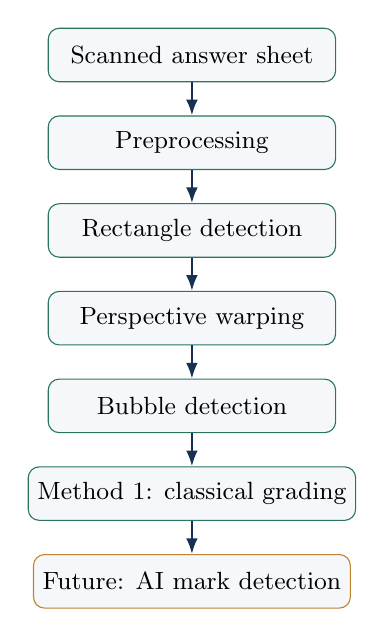
\begin{tikzpicture}[
    node distance=0.42cm,
    stage/.style={
      rectangle,
      rounded corners,
      draw=projectblue,
      fill=softgray,
      minimum width=3.65cm,
      minimum height=0.68cm,
      align=center,
      font=\small
    },
    done/.style={
      rectangle,
      rounded corners,
      draw=projectgreen,
      fill=softgray,
      minimum width=3.65cm,
      minimum height=0.68cm,
      align=center,
      font=\small
    },
    future/.style={
      rectangle,
      rounded corners,
      draw=projectgold,
      fill=softgray,
      minimum width=3.65cm,
      minimum height=0.68cm,
      align=center,
      font=\small
    },
    arrow/.style={-{Latex[length=2mm]}, thick, projectblue}
  ]
    \node[done] (input) {Scanned answer sheet};
    \node[done, below=of input] (pre) {Preprocessing};
    \node[done, below=of pre] (rects) {Rectangle detection};
    \node[done, below=of rects] (warp) {Perspective warping};
    \node[done, below=of warp] (bubbles) {Bubble detection};
    \node[done, below=of bubbles] (method1) {Method 1: classical grading};
    \node[future, below=of method1] (ai) {Future: AI mark detection};

    \draw[arrow] (input) -- (pre);
    \draw[arrow] (pre) -- (rects);
    \draw[arrow] (rects) -- (warp);
    \draw[arrow] (warp) -- (bubbles);
    \draw[arrow] (bubbles) -- (method1);
    \draw[arrow] (method1) -- (ai);
  \end{tikzpicture}
\end{frame}

\begin{frame}{Stage 1: Preprocessing}
  \begin{columns}[T]
    \begin{column}{0.48\textwidth}
      \textbf{Goal}
      \begin{itemize}
        \item standardize image size,
        \item convert to grayscale,
        \item smooth small noise,
        \item extract strong edges.
      \end{itemize}

      \vspace{0.2cm}

      This step prepares the sheet for layout detection while keeping the process simple enough to inspect in the notebook.
    \end{column}
    \begin{column}{0.48\textwidth}
      \centering
      \maybeimage[width=\linewidth]{samples/canny_File0005.png}

      \vspace{0.08cm}
      \small Canny output used as a visual checkpoint.
    \end{column}
  \end{columns}
\end{frame}

\begin{frame}{Stage 2: Reference Rectangle Detection}
  \begin{block}{Why rectangles are central}
    The sheet is not searched blindly. The large printed rectangles define stable regions of interest: the answer area and the ID area.
  \end{block}

  \begin{columns}[T]
    \begin{column}{0.52\textwidth}
      \textbf{Implementation}
      \begin{itemize}
        \item threshold the sheet for dark structures,
        \item find external contours,
        \item keep rectangle-like contours,
        \item select the two largest rectangles.
      \end{itemize}
    \end{column}
    \begin{column}{0.42\textwidth}
      \textbf{Why it matters}
      \begin{itemize}
        \item reduces search area,
        \item normalizes downstream steps,
        \item creates clear debugging checkpoints.
      \end{itemize}
    \end{column}
  \end{columns}
\end{frame}

\begin{frame}{Stage 3: Perspective Correction}
  \begin{columns}[T]
    \begin{column}{0.46\textwidth}
      \textbf{Largest rectangle}

      \vspace{0.12cm}
      The largest detected rectangle is treated as the answer section. Its four corners are ordered and warped into a normalized rectangular image.

      \vspace{0.25cm}

      This makes the bubble rows easier to compare because geometry becomes more regular.
    \end{column}
    \begin{column}{0.50\textwidth}
      \centering
      \maybeimage[height=0.72\textheight]{samples/stage_outputs/rectangle_1_warped.png}
    \end{column}
  \end{columns}
\end{frame}

\begin{frame}{Stage 4: Bubble Candidate Detection}
  \begin{columns}[T]
    \begin{column}{0.44\textwidth}
      \textbf{Classical detection}
      \begin{itemize}
        \item Hough circles propose bubble candidates.
        \item A color filter removes many false positives for this template.
        \item Dark-pixel ratio estimates whether a bubble is marked.
      \end{itemize}

      \vspace{0.2cm}
      \small Green circles are candidates. Red circles pass the mark threshold.
    \end{column}
    \begin{column}{0.52\textwidth}
      \centering
      \maybeimage[height=0.72\textheight]{samples/stage_outputs/rectangle_1_bubbles.png}
    \end{column}
  \end{columns}
\end{frame}

\begin{frame}{Method 1: Classical Answer Interpretation}
  \begin{block}{What was added after bubble detection}
    Detected bubbles are no longer only visual candidates. They are ordered, grouped, interpreted, and compared with an answer key.
  \end{block}

  \begin{columns}[T]
    \begin{column}{0.49\textwidth}
      \textbf{Grouping}
      \begin{itemize}
        \item cluster bubble centers by x-position,
        \item split 12 option columns into 3 answer blocks,
        \item group rows inside each block,
        \item map four bubbles to A, B, C, D.
      \end{itemize}
    \end{column}
    \begin{column}{0.45\textwidth}
      \textbf{Decision labels}
      \begin{itemize}
        \item \texttt{A-D}: one clear mark,
        \item \texttt{X}: blank answer,
        \item \texttt{M}: multiple marks,
        \item \texttt{?}: unclear, review needed.
      \end{itemize}
    \end{column}
  \end{columns}
\end{frame}

\begin{frame}{Human Review Is a Feature}
  \begin{block}{Trustworthy grading}
    A useful grading assistant should not force a decision when the evidence is weak. It should separate confident answers from cases that require a teacher or operator.
  \end{block}

  \begin{table}
    \centering
    \begin{tabular}{lll}
      \toprule
      Case & Output & Meaning \\
      \midrule
      one strong mark & A, B, C, or D & normal answer \\
      no mark & X & blank answer \\
      two or more marks & M & multiple marks detected \\
      weak or ambiguous mark & ? & unclear, please review \\
      \bottomrule
    \end{tabular}
  \end{table}

  \vspace{0.1cm}
  \small This is important for real classrooms, where erasures, faint marks, and accidental double marks happen.
\end{frame}

\begin{frame}{Current Evaluation Checkpoint}
  \begin{columns}[T]
    \begin{column}{0.31\textwidth}
      \metric{Option columns}{12}
    \end{column}
    \begin{column}{0.31\textwidth}
      \metric{Answer blocks}{3}
    \end{column}
    \begin{column}{0.31\textwidth}
      \metric{Rows detected}{100}
    \end{column}
  \end{columns}

  \vspace{0.2cm}

  \begin{table}
    \centering
    \begin{tabular}{lcc}
      \toprule
      Output type & Count & Comment \\
      \midrule
      interpreted answers & 100 & all rows grouped successfully \\
      review flags & 0 & current clean sample only \\
      generated report & yes & JSON output for grading results \\
      \bottomrule
    \end{tabular}
  \end{table}

  \small The current score uses a demo answer key, so it proves the grading pipeline works but should not be interpreted as a real student grade.
\end{frame}

\begin{frame}{What Is Implemented Now}
  \begin{columns}[T]
    \begin{column}{0.48\textwidth}
      \textbf{Code modules}
      \begin{itemize}
        \item preprocessing helpers,
        \item contour and rectangle detection,
        \item bubble candidate detection,
        \item classical grading method,
        \item editable answer-key JSON.
      \end{itemize}
    \end{column}
    \begin{column}{0.48\textwidth}
      \textbf{Notebooks}
      \begin{itemize}
        \item preprocessing tests,
        \item contour detection,
        \item bubble detection,
        \item classical grading.
      \end{itemize}
    \end{column}
  \end{columns}

  \vspace{0.35cm}

  \begin{block}{Academic value}
    The project is organized as a reproducible pipeline, where every stage can be visualized, inspected, and replaced.
  \end{block}
\end{frame}

\begin{frame}{Limitations and Risks}
  \begin{itemize}
    \item Current tests are still based on a small number of sample sheets.
    \item The color filter is useful for the current orange-bubble template, but other templates may need it disabled.
    \item Thresholds are understandable, but they still require evaluation on more scans.
    \item The system currently processes the answer section first; ID extraction is prepared but not final.
    \item A real answer key is required before reporting meaningful student grades.
  \end{itemize}

  \vspace{0.3cm}

  \begin{block}{Why this honesty matters}
    In computer vision, a strong project is not only one that works on a demo image. It is one that knows what it can trust, what it cannot trust yet, and how to test the difference.
  \end{block}
\end{frame}

\begin{frame}{Next Research Steps}
  \begin{enumerate}
    \item Test sheets with blank, faint, erased, and multiple-mark answers.
    \item Replace the demo key with real teacher answer keys.
    \item Add ID-section interpretation.
    \item Evaluate Method 1 with clear metrics:
      \begin{itemize}
        \item question-level accuracy,
        \item exact-sheet accuracy,
        \item review rate,
        \item runtime per sheet.
      \end{itemize}
    \item Develop and compare an AI-based mark detector.
  \end{enumerate}
\end{frame}

\begin{frame}{Expected Impact}
  \begin{block}{For low-resource schools}
    A scanner and a laptop could become enough to reduce hours of repetitive grading work, while still keeping teachers in control of uncertain answers.
  \end{block}

  \vspace{0.2cm}

  \begin{columns}[T]
    \begin{column}{0.48\textwidth}
      \textbf{Practical impact}
      \begin{itemize}
        \item faster grading,
        \item lower cost,
        \item repeatable scoring,
        \item review-aware reports.
      \end{itemize}
    \end{column}
    \begin{column}{0.48\textwidth}
      \textbf{Academic impact}
      \begin{itemize}
        \item classical baseline,
        \item future AI comparison,
        \item explainable pipeline,
        \item measurable robustness.
      \end{itemize}
    \end{column}
  \end{columns}
\end{frame}

\begin{frame}{Conclusion}
  \begin{block}{Current achievement}
    We built a modular computer vision pipeline that detects answer-sheet regions, warps them, detects bubble candidates, and now interprets answer rows using a classical grading method.
  \end{block}

  \vspace{0.25cm}

  The project is not finished yet. The current result is a strong baseline: explainable, visual, and ready for systematic evaluation against future AI-based methods.

  \vspace{0.3cm}

  \centering
  \Large From scanned paper to review-aware grading.
\end{frame}

\begin{frame}
  \centering
  \Huge Thank you

  \vspace{0.45cm}

  \Large Questions?
\end{frame}

\end{document}
